\chapter{Design and Implementation}

\section{Trainer Interface: The Website}
The following are screenshots of the website we designed and built for the trainers. These five images show the main pages of our website: Home, Add a User, Training Materials, Assign Training Material, and Message Log. The goal is a clean, simple interface that is intuitive and functional. Additional screenshots from the website are included in the Appendices.

\begin{figure}[H]
	\centering
	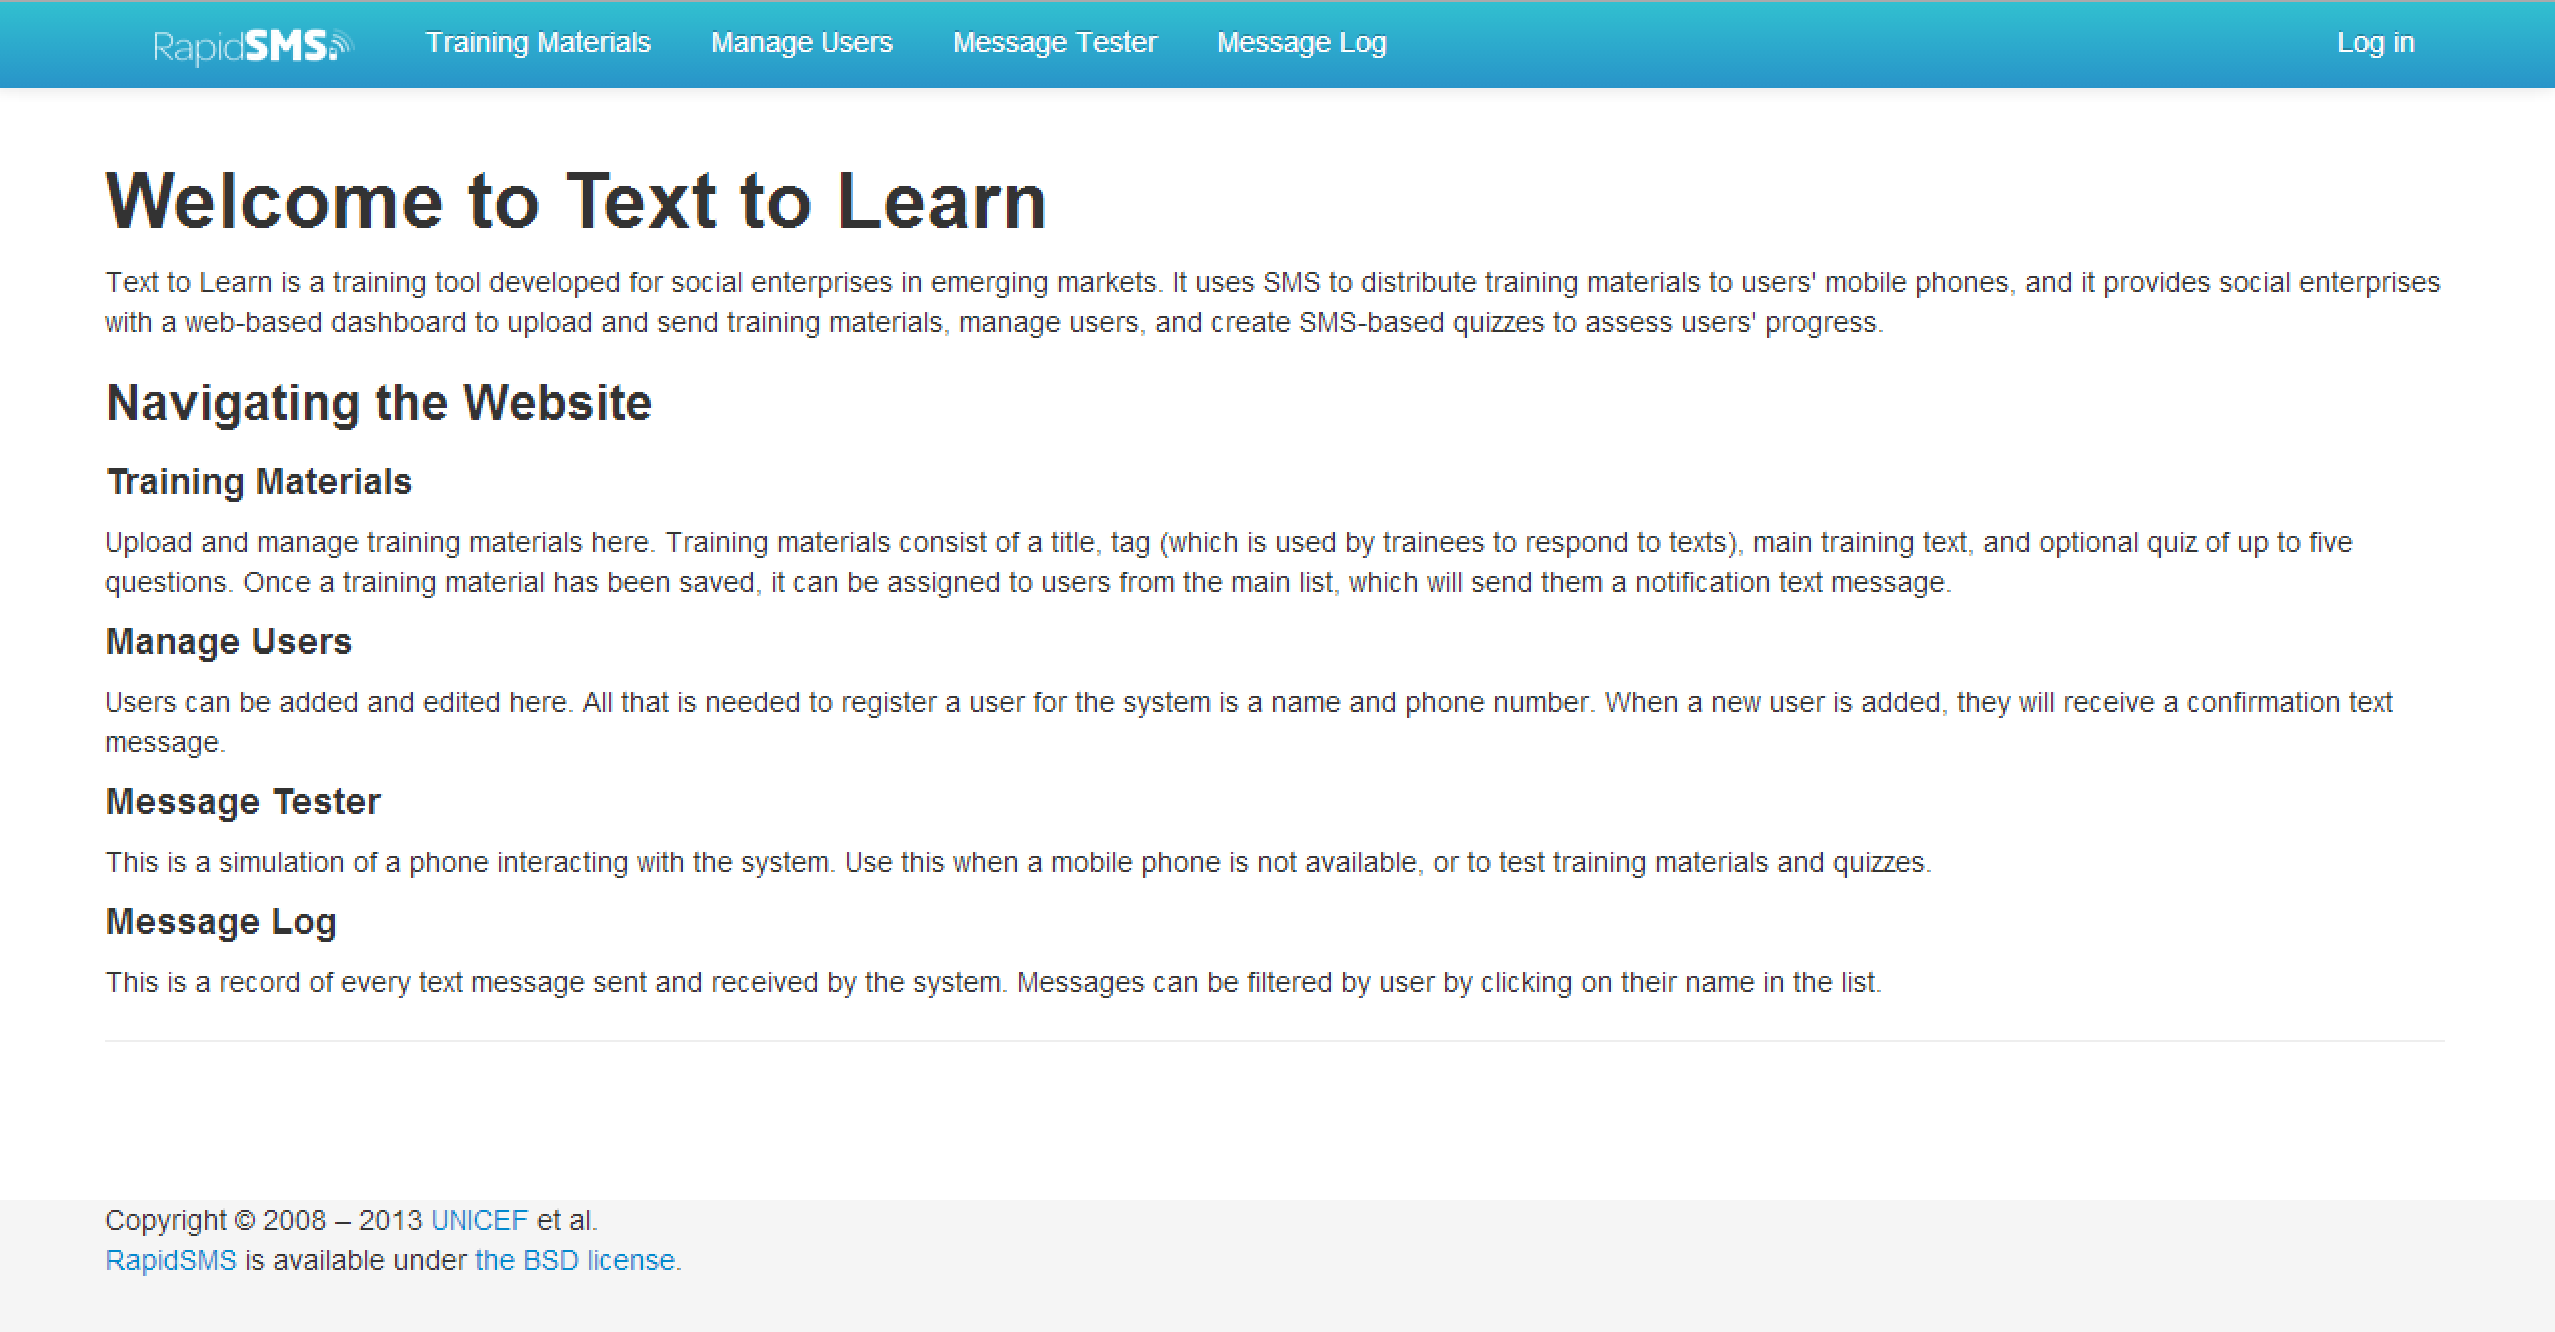
\includegraphics[scale=0.15]{home.png}
	\caption{Home page}
\end{figure}

\begin{figure}[H]
	\centering
	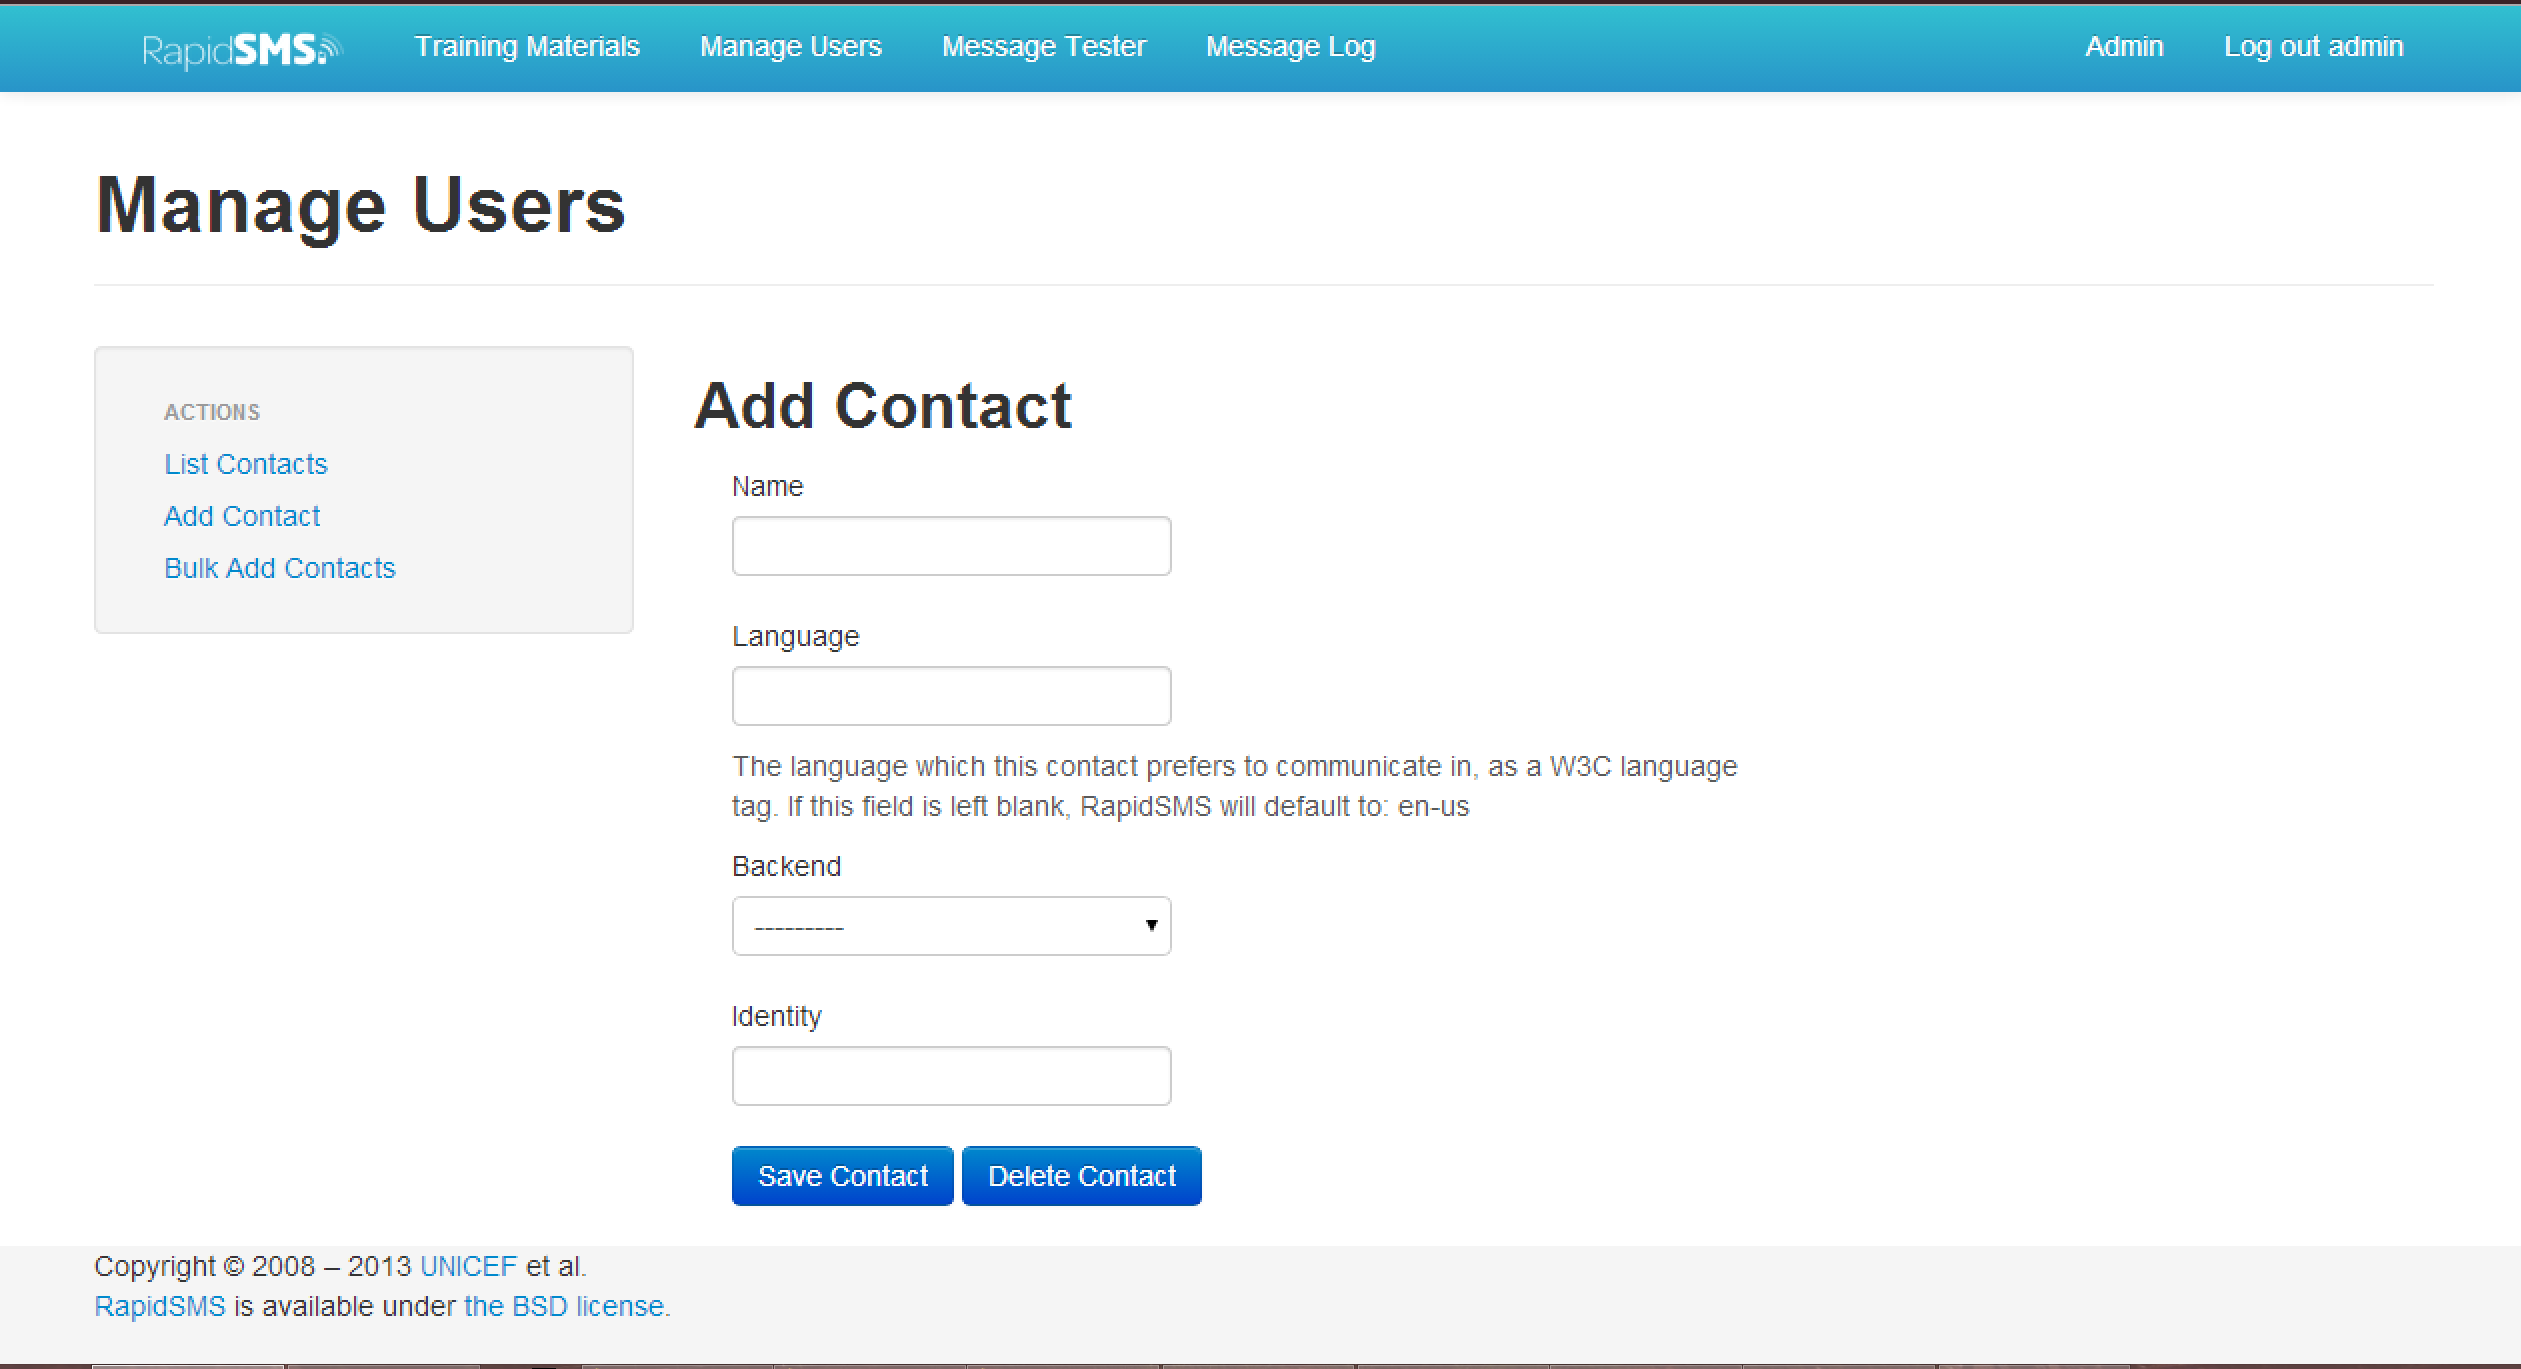
\includegraphics[scale=0.15]{add_contact.png}
	\caption{Add a User}
\end{figure}

\begin{figure}[H]
	\centering
	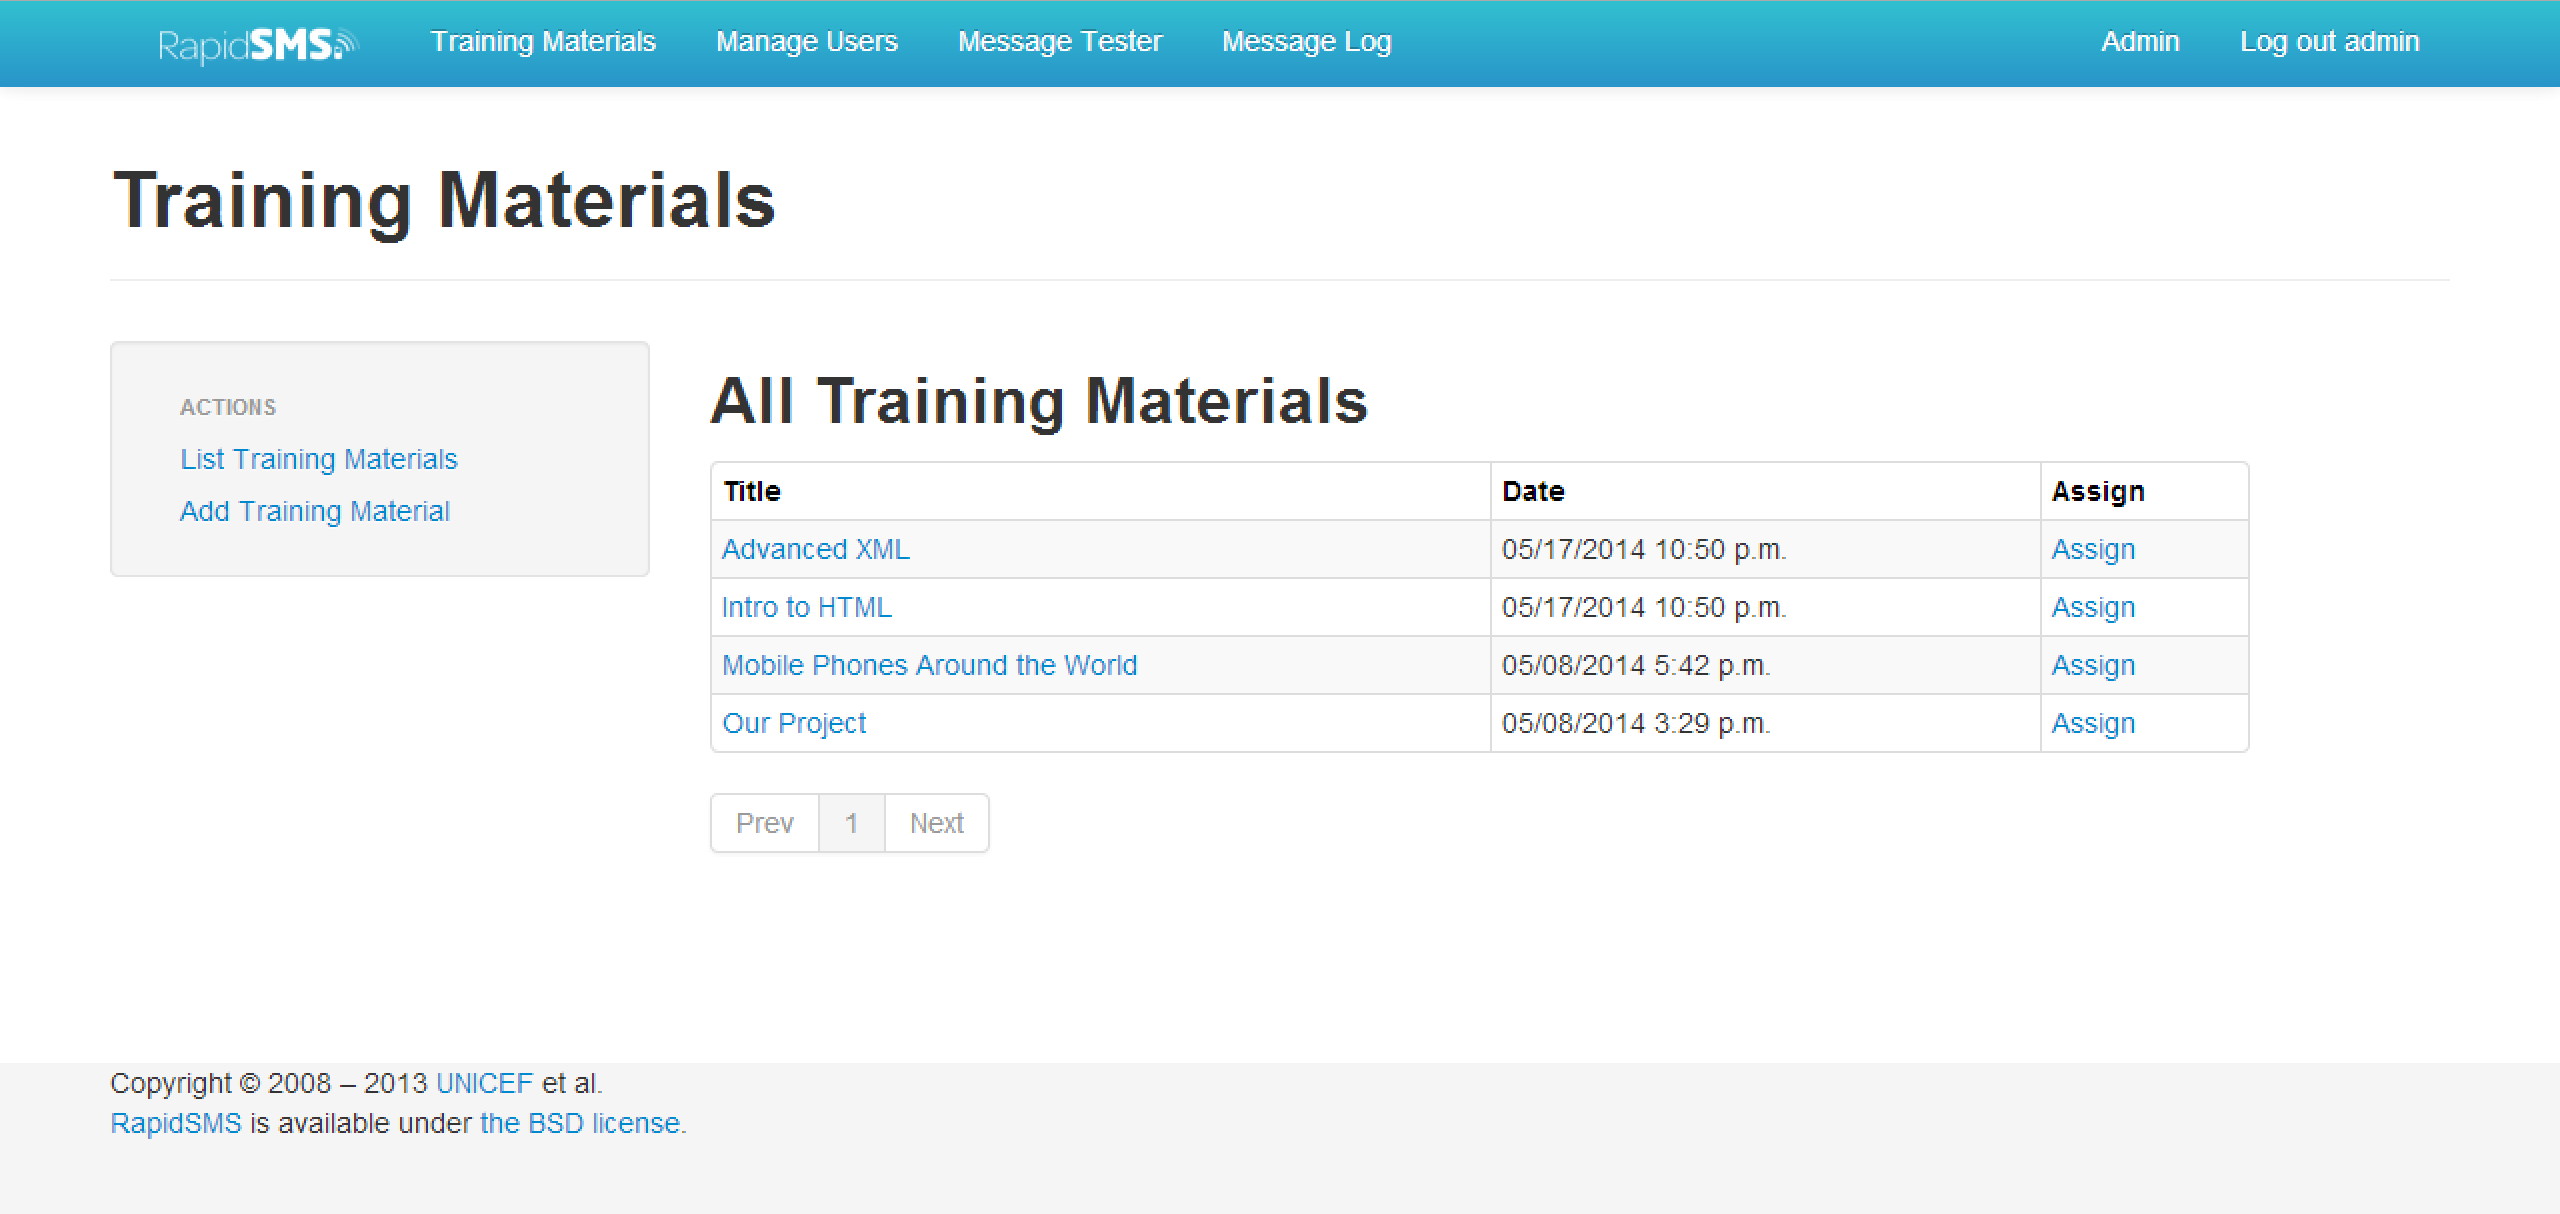
\includegraphics[scale=0.15]{list_tm.png}
	\caption{Training Materials}
\end{figure}

\begin{figure}[H]
	\centering
	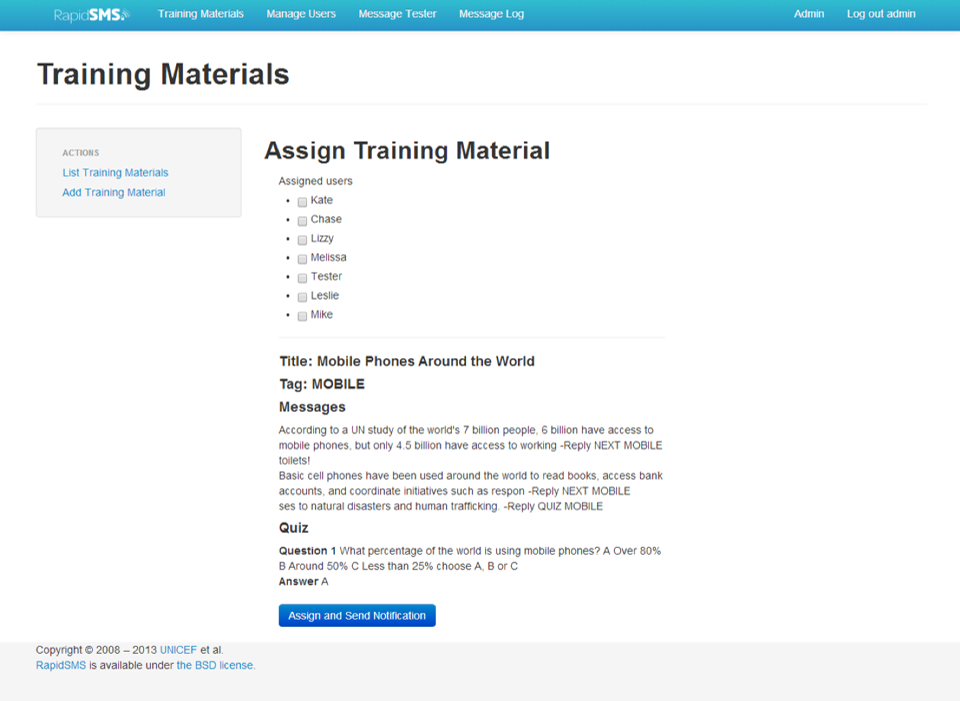
\includegraphics[scale=0.62]{assign_tm.png}
	\caption{Assign Training Material to Users}
\end{figure}

\begin{figure}[H]
	\centering
	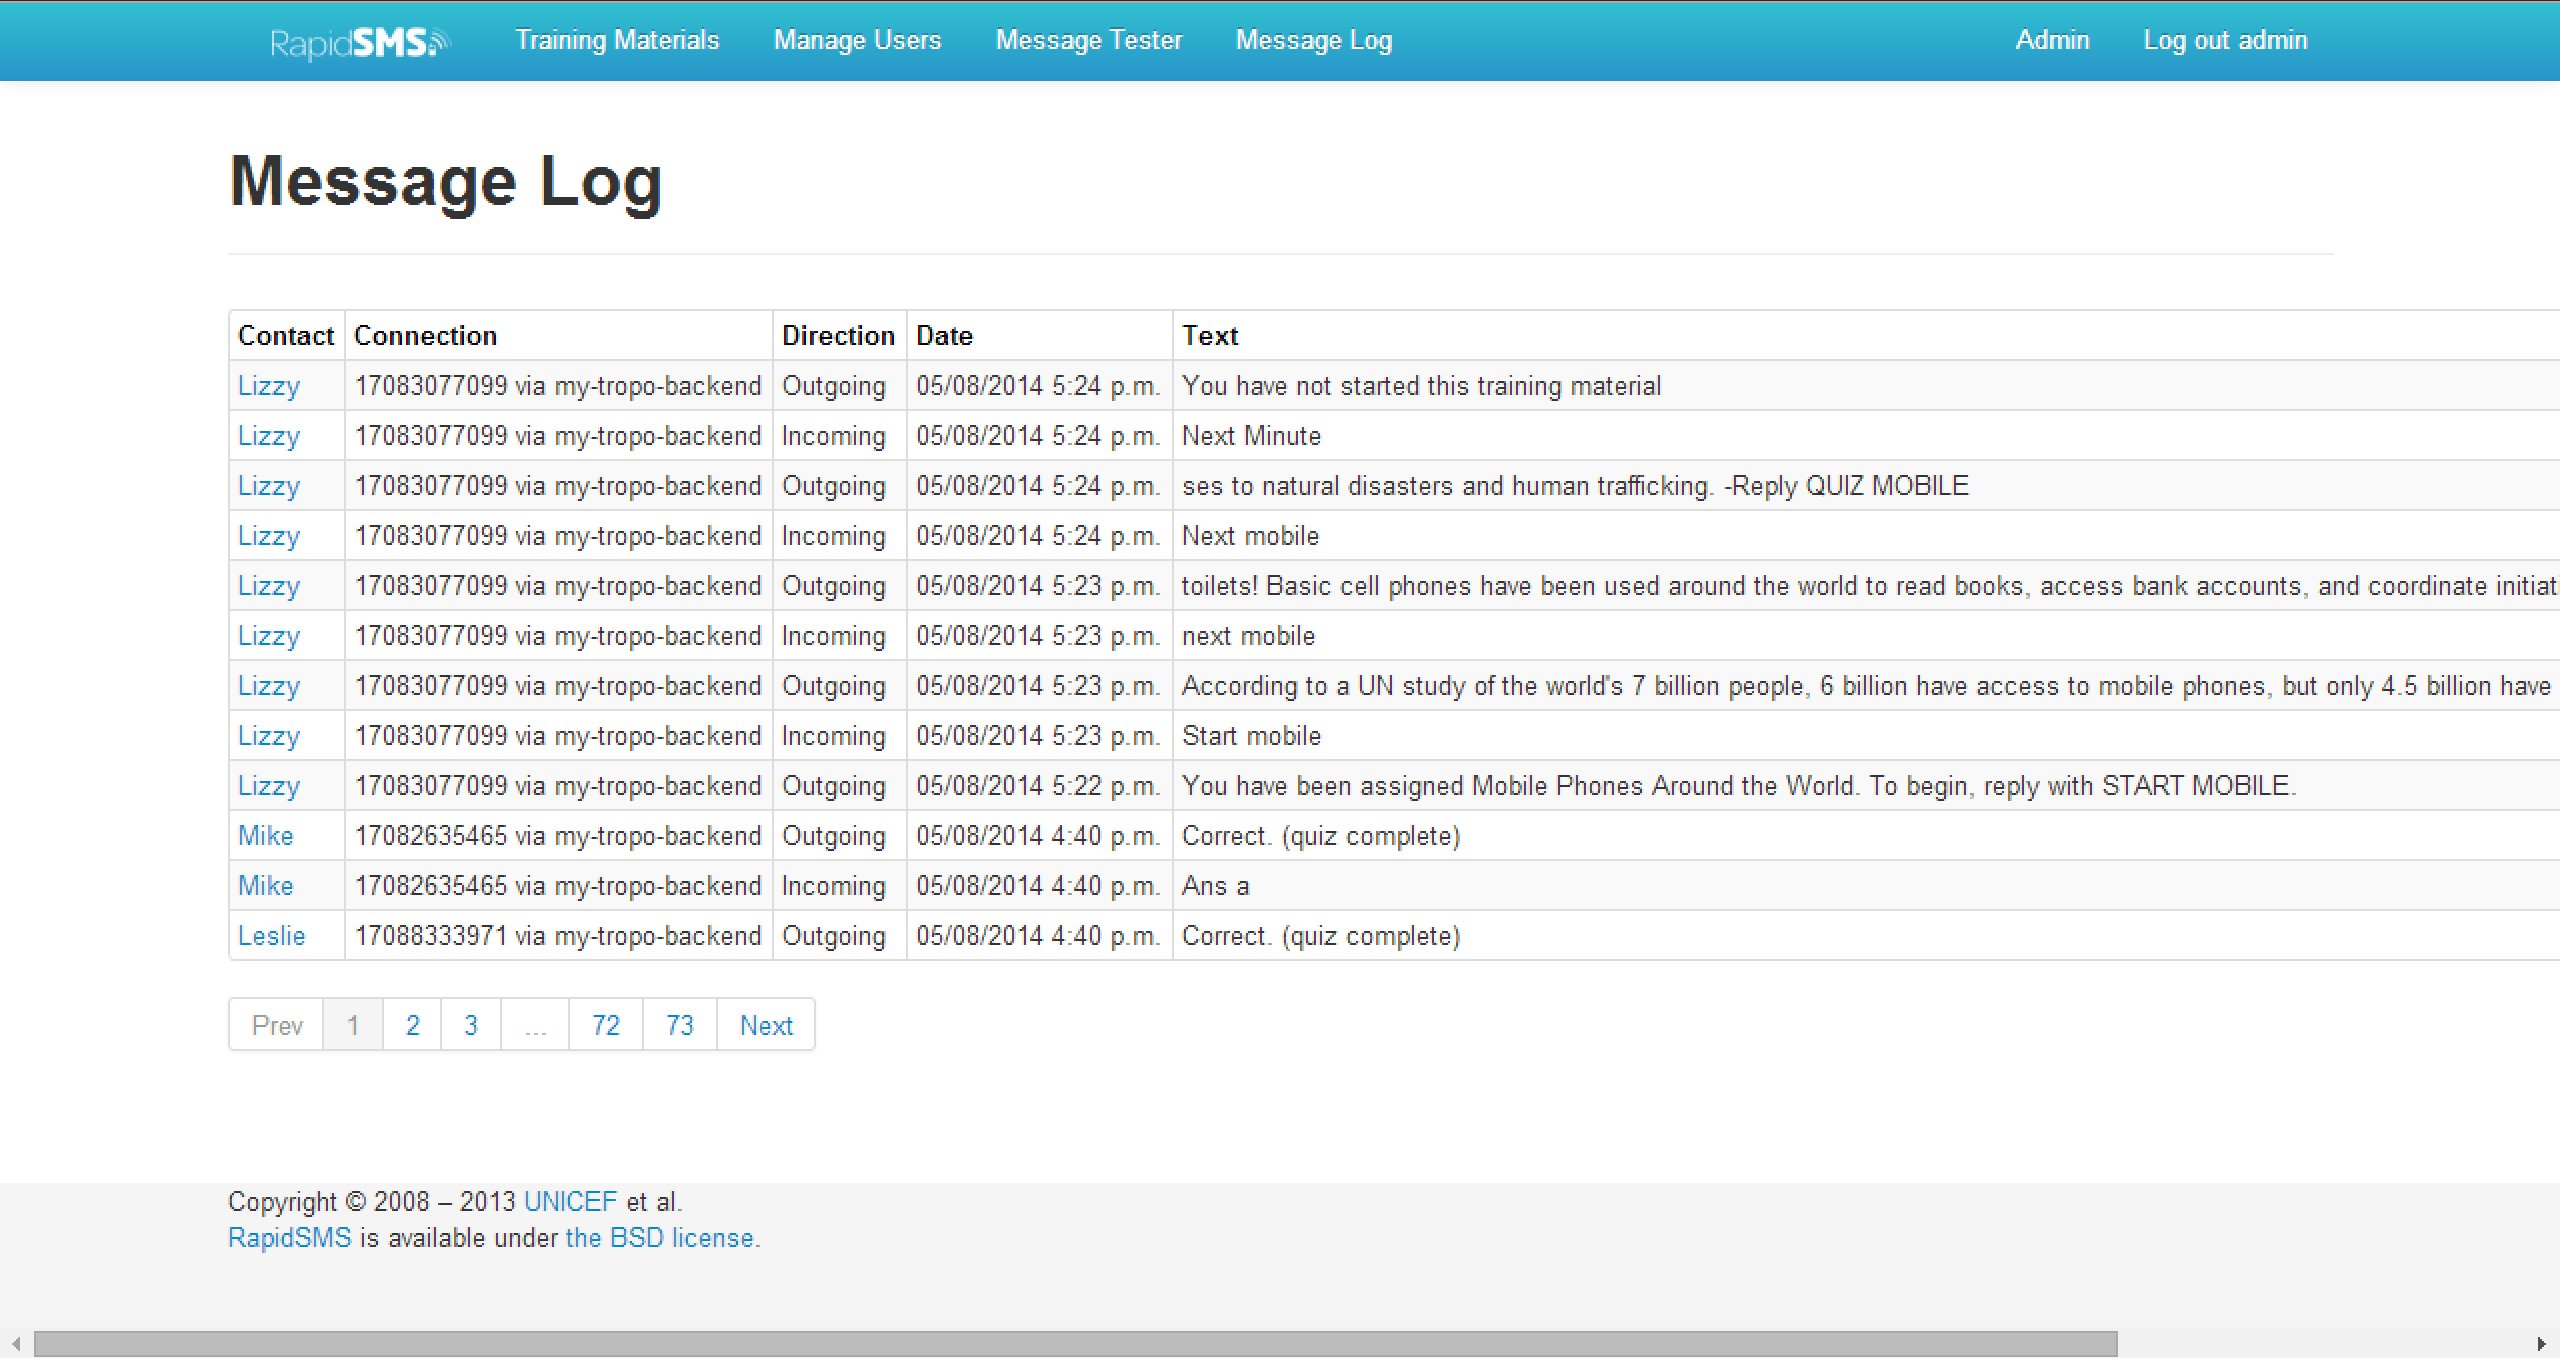
\includegraphics[scale=0.15]{message_log.png}
	\caption{Message Log}
\end{figure}


\section{Trainee Interaction: The Phone}
Trainees, or the users that are registered for Text to Learn, interact with the system through their mobile phones via SMS text messaging. Once their phone number has been registered by a trainer, they are able to text the Text to Learn phone number. At any time, a user can get help for using our system using the \textit{HELP} command.


\begin{table}[H]

    \begin{tabular}{ | p{5cm} | p{7cm} |}
    \hline
    \textbf{Status} & \textbf{Text Received by Trainee} \\ \hline
    Once assigned a training material & You have been assigned <training material name>. To begin, reply with START <TM tag>.  \\ \hline
    After starting a training material & 9C  \\ \hline
    At final message of training material with a quiz & 10C \\ \hline
    At final message of training material without a quiz & 9C  \\ \hline
    At final message of quiz & 9C  \\ \hline
	\end{tabular}
	\caption{Table taken from}
\end{table}
	

\section{System Design}
The following diagrams show our design visually by specifying the three main components of our system (webpage, cloud storage, and SMS service), the main functionality of each component, and how they interact with each other.

Our system is designed around three main components: a website, SMS, and cloud storage. The website is the way trainers or distributors interact with the system. Through the website, trainers can login to the office of their choosing and manage users, add new training materials and quizzes, and view, edit, and manage previously uploaded training materials and quizzes. To add users, the trainer simply needs to know the trainee's phone number and add it into the system. Adding new training materials and quizzes requires trainers to have these in plain text format and then copy and paste them into the appropriate text fields. From there, the materials can be assigned and sent to trainees via SMS. Through the website's message log, the trainers are able to view every message sent and received by the system, and filter this by user to see a particular user's responses to a quiz.

\begin{figure}[H]
	\centering
	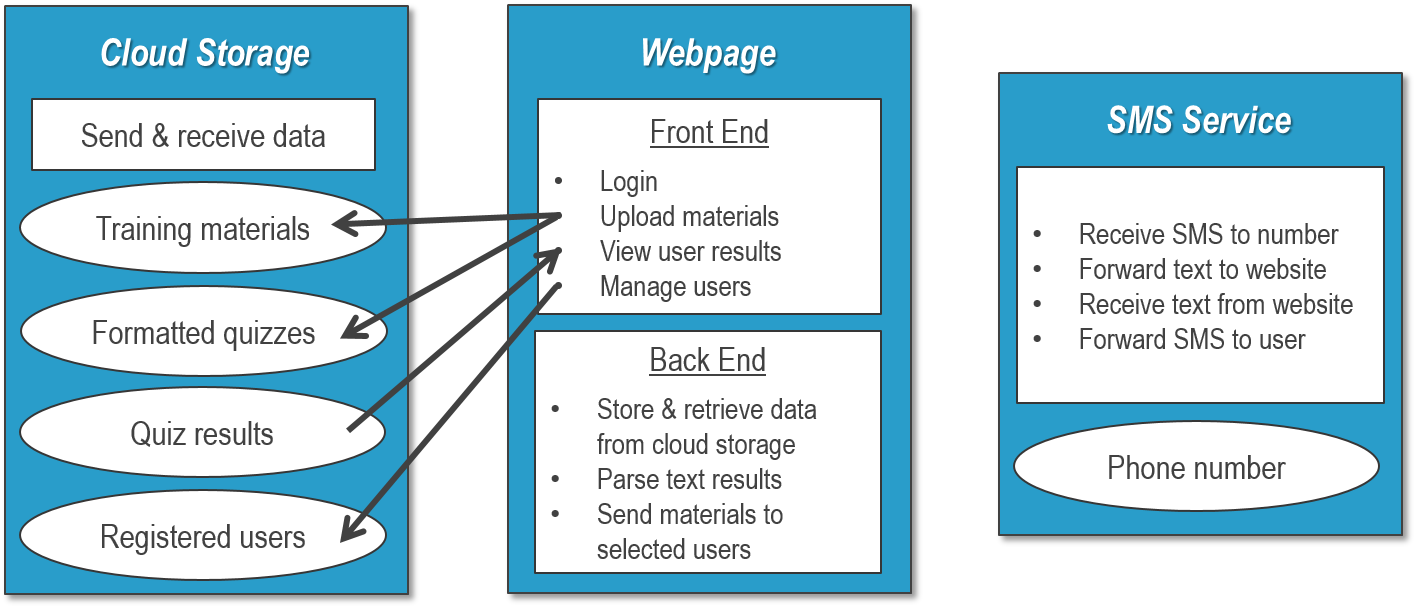
\includegraphics[scale=0.5]{trainer.png}
	\caption{System Diagram for Trainer}
\end{figure}

Trainees will interact with the system through SMS. ...

\begin{figure}[H]
	\centering
	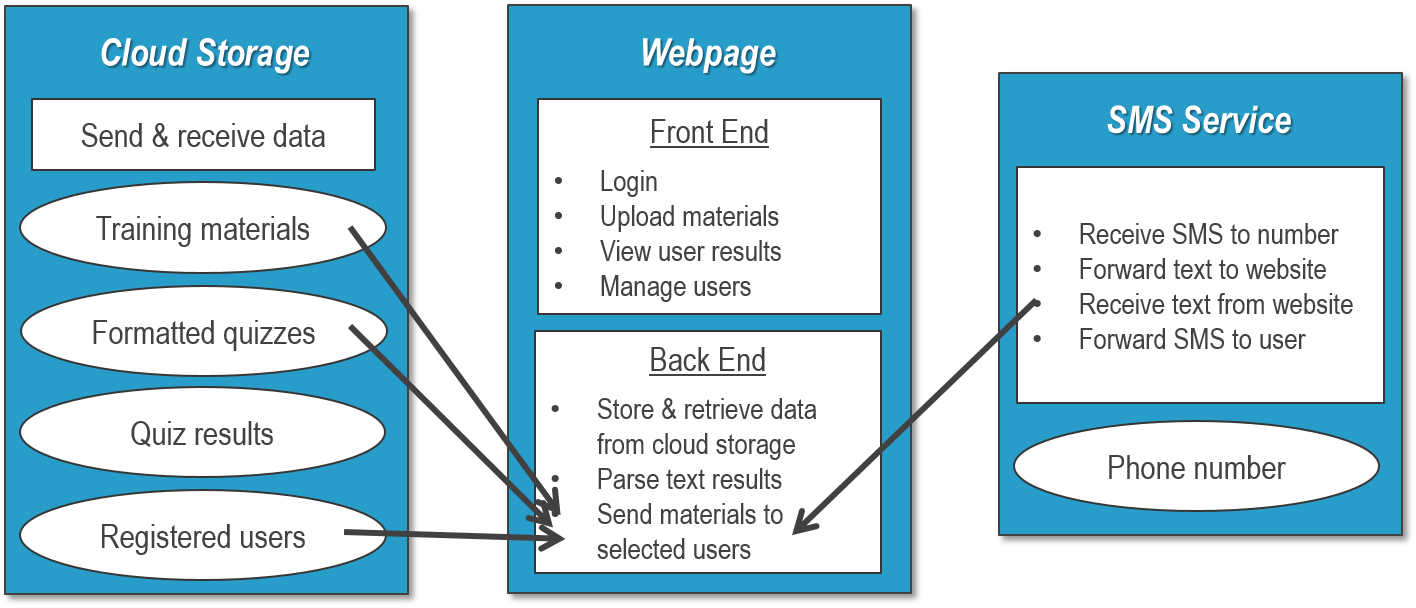
\includegraphics[scale=0.5]{trainee_request.png}
	\caption{System Diagram for Trainee Request}
\end{figure}

\begin{figure}[H]
	\centering
	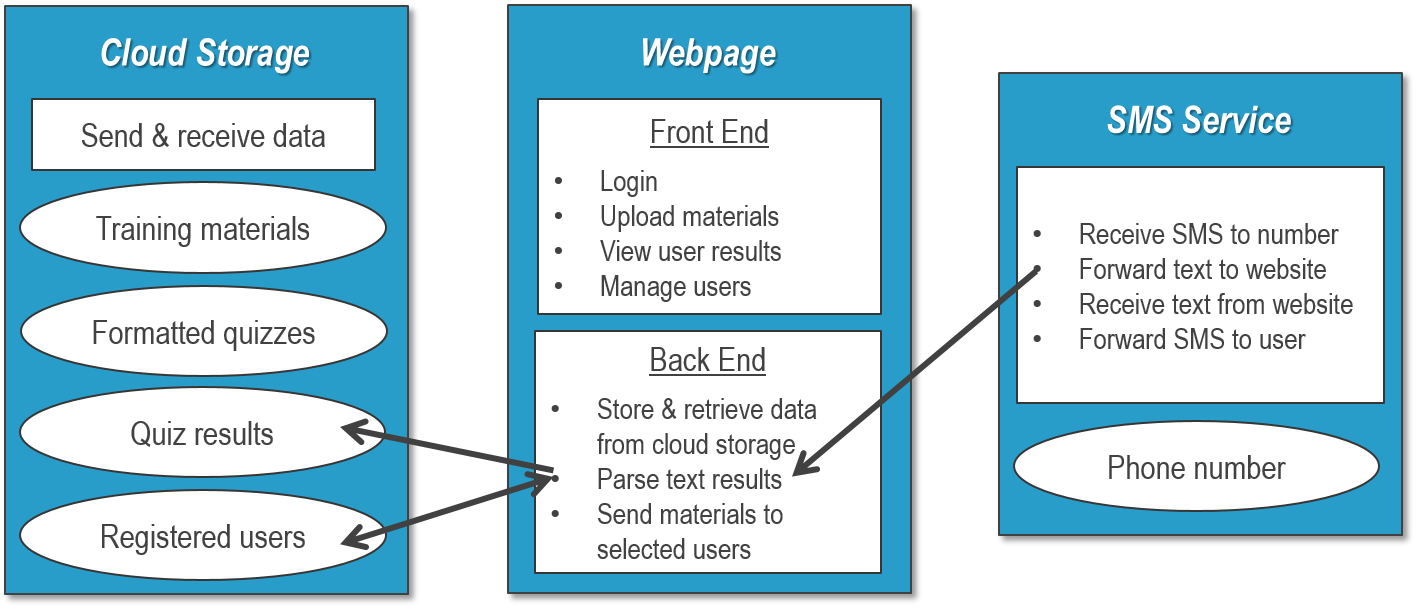
\includegraphics[scale=0.5]{trainee.png}
	\caption{System Diagram for Trainee}
\end{figure}

\section{Technologies Used}
\begin{description}
	\item[RapidSMS] a recent UNICEF project built to integrate SMS services with the Django web-framework
	\begin{description}
		\item[Django] a web-framework that lends itself to form collections
		\item[Python] the primary programming language used in Django
	\end{description}
	\item[dotCloud] a cloud web-hosting service that hosts our website in a Python web server and our data in a PostgreSQL database
	\item[Tropo] a web-based SMS service that generates a phone number and API to connect to websites
	\item[GitHub] version control system
\end{description}

\section{Design Rationale}

We chose to use a cloud service for storage rather than a local server. The cloud service holds all of the information that is sent and received between trainers and trainees, including training documents, formatted quizzes, quiz results, and registered users. Storing information “in the cloud” means that it can be accessed by other people directly through the internet, so trainers have access to this information from any computer with internet connection, whether at the office or at home. The cloud offers storage for large amounts of data, so trainers will not be limited by storage space when uploading training materials. The alternative to using cloud storage would be to have all of the training materials stored on a server belonging to the individual social enterprise. We decided against this option because cloud computing is the technology of the future. Although all social enterprises may not have the capability to use cloud services at their offices currently, cloud computing is growing rapidly in popularity and is sure to be utilized by more social enterprises eventually.

We considered building our system as a native phone apps, however we saw more barriers to this approach versus an SMS-based system. Since our target audience will often have the most basic phones, their phones may not be able to support even Java applications that are available on most feature phones, and would require use of the internet which again is often not supported. Even if these problems were not a barrier, the application would need to be installed on the phone, and not all phones have a way to install applications via the Web and may require the phone owner to go to their office to install the application. Essentially, using SMS has virtually no startup costs, and it will reach the broadest audience possible in emerging markets.

The system will also be using a paid SMS service to manage incoming and outgoing texts. While we could have written scripts to send texts from an email address for free, we would have needed to know the user’s service provider, and that service provider must have an email domain which may not be extensible to developing countries. There are open source models that work by plugging a gsm modem with a sim card into a computer to receive texts, but these are often difficult to work with and hard to scale. For these reasons, we made the decision to use a paid SMS service rather than using an email address to handle text messaging.
